\documentclass[10pt]{article}
\usepackage{graphicx,amssymb, amstext, amsmath, epstopdf, booktabs, verbatim, gensymb, geometry, appendix, lmodern}
\geometry{letterpaper}

\newcommand*\Title{Rapport de stage de fin d'études}
\newcommand*\subtitle{Sécurité, CI \& développement Java}
\newcommand*\Date{\today}
\newcommand*\Author{Alexandre Léonardi}
\title{Rapport de stage de fin d'études}
\author{Alexandre Léonardi}
\date{\today}
%-----------------------------------------------------------

\usepackage{cpistuff/cpi} % This is what makes your document look like a cpi document.

\addbibresource{parts/references.bib} 

\begin{document}

\begin{titlepage}
	\maketitle
\end{titlepage}

\linespread{1.15} %Set standard document linespacing

\setcounter{tocdepth}{2}
\tableofcontents
\addtocontents{toc}{~\hfill\textbf{Page}\par}
\pagebreak
\section*{Introduction}
Développement Java et développement d'une solution d'analyse statique de sécurité : ce sont les deux principales branches de mon stage. Il s'agit pour partie de prendre part aux contrats en Java d'Alter Frame, l'entreprise qui m'accueille pour la durée du stage, et d'autre part d'intervenir sur un projet en interne visant à mettre en place une analyse de sécurité systématique des projets Web au-travers de pratiques de CI\cite{ci_wiki}\footnote{Continuous Integration ou intégration continue}. 

Ce sujet a l'avantage d'être ouvert et diversifié. Il me permet d'une part de travailler sur du pur développement et d'autre part de mettre en pratique la composante sécurité de la formation FSI\cite{fsi}\footnote{Fiabilité et sécurité informatique}, tout en découvrant les concepts de CI qui m'étaient jusque là étrangers, ainsi que des technologies qui vont de pair telles que Docker.

En pratique, un troisième pan viendra s'ajouter à mon sujet de stage : un audit technique pour un client d'Alter Frame souhaitant des pistes d'amélioration de son application, notamment en termes de qualité de code. 

À noter que, par discrétion à leur égard, les noms des clients d'Alter Frame ne seront pas mentionnés et seront effacés des captures d'écran que vous trouverez dans ce document. Il en ira de même pour les différents projets.
\pagebreak
\section{Présentation d'Alter Solutions Engineering} 
Alter Solutions Engineering, et plus particulièrement sa filiale Alter Frame, est l'entreprise qui m'a accueilli pour la durée de mon stage de fin d'études, nous allons donc commencer par la présenter rapidement.

\subsection{Les subdivisions d'Alter Solutions Engineering et leurs secteurs d'activité}
Alter Solutions Engineering est une entreprise relativement jeune : elle a été créée en 2006 et, si elle n'entre plus maintenant dans la catégorie des PME en termes de nombre de collaborateurs, elle reste une structure de petite taille.

Le siège social de l'entreprise se trouve à Versailles et c'est là où travaille l'équipe de développement française dont je fais partie. En pratique, il s'agit de l'équipe de développement d'Alter Frame qui est une entité enfant d'Alter Solutions Engineering (cf. section~\ref{subsec:frame}).

Alter Solutions Engineering est une société de conseil en hautes technologies mais en pratique, elle est composée de trois filières qui ont chacune une spécialité bien distinctes (cf. graphique~\ref{fig:filiales}).
\begin{figure}
  \centering
  \caption{Alter Solutions Engineering et ses filiales}
  \label{fig:filiales}
  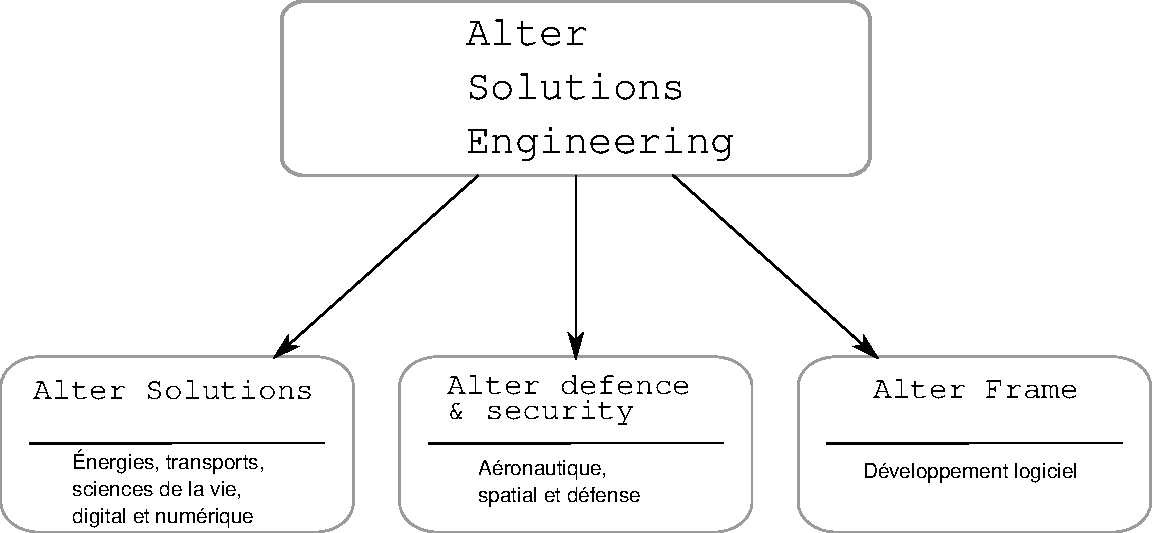
\includegraphics[width=\textwidth]{images/filiales_allinone.pdf}
\end{figure}

\subsubsection{Alter Solutions}
Cette filiale est spécialisée dans le conseil en ingénierie, notamment dans les domaines de l'énergie, des transports, des sciences de la vie, du digital et du numérique.

\subsubsection{Alter defence \& security}
Alter defence est également orientée vers le conseil, mais cette fois plus particulièrement dans l'aéronautique, le sptial et la défense.
  
\subsubsection{Alter Frame}
Alter Frame enfin est la branche spécialisée dans l'édition de logiciels et celle que j'ai rejoint durant mon stage. C'est une ESN\footnote{Entreprise de Services du Numérique, cf. \url{https://fr.wikipedia.org/wiki/Entreprise_de_services_du_num\%C3\%A9rique}} dont l'activité est elle-même répartie en deux catégories :
\begin{itemize}[label=$\bullet$]
\item le conseil, c'est-à-dire le fait de fournir des spécialistes d'un domaine du numérique pour la durée d'un contrat à un client ;
\item le développement de logiciels au forfait, c'est-à-dire le fait de prendre commande d'un logiciel à réaliser en interne et de le livrer à la fin du contrat.
\end{itemize}

\subsection{Un peu plus de détails sur Alter Frame}
\label{subsec:frame}
Bien qu'Alter Frame ait des clients et des domaines d'intervention variés, en termes de technologes il y a trois pôles de compétences qui sont caractéristiques de l'entreprise et reviennent le plus régulièrement :
\begin{itemize}[label=$\bullet$]
\item Java ;
\item .NET ;
\item PHP.
\end{itemize}

Mon stage ne s'est pas cantonné au domaine du développement mais il en a tout de même inclus celui-ci s'est déroulé au sein de l'équipe Java.
    
\subsection{Quelques (derniers) chiffres}
TODO : À remettre en forme pour plus tard
Mettre une note\footnote{\url{http://www.alter-solutions.com/notre-societe/chiffres-cles/}}.
375 collaborateurs en France, Portugal et Belgique (combien dans chaque pays ?)

\subsection{Répartition de l'activité}
\begin{tikzpicture}
    \pie[color ={ cyan!10 , cyan!20, cyan!30,  cyan!40}, explode=0.1]{10/A, 20/B, 30/C, 40/D}
\end{tikzpicture}

\pagebreak
\section{Retour d'expérience sur mon stage}
\pagebreak
\section{Environnement de travail \& solutions retenues}
Je ne suis intervenu que sur des projets qui étaient déjà commencés, et de ce fait il n'y a eu que peu de choix en termes de solutions retenues. Je vais néanmoins détailler ici l'environnement de travail, les différentes solutions techniques qui étaient déjà en place à mon arrivée et avec lesquelles j'ai travaillé pendant 6 mois.

Pour autant, il est intéressant de résumer l'environnement dans lequel j'ai évolué pendant 6 mois, pour chacun des pans très variés sur lesquels je suis intervenu. Les sous-sections seront volontairement brèves ; plus de détails seront disponibles dans les parties~\ref{sec:synthese_ci},~\ref{sec:synthese_java} et~\ref{sec:synthese_audit}.

\subsection{CI}
\subsubsection{GitLab \& GitLab-CI}
L'intégration continue dans les projets d'Alter Frame se fait à l'aide d'un service proposé par la plateforme d'hébergement de projets informatiques GitLab\cite{gitlab}. Le service en question, GitLab-CI\cite{gitlab-ci}, propose de mettre en place de l'intégration continue sur les projets hébergés sur GitLab.

Au moment de mon arrivée chez Alter Frame la partie CI des projets consistait majoritairement en la compilation des projets et une analyse de code à l'aide d'un plugin SonarQube\cite{sonarqube}, mise en place depuis environ 2 ans.

Le principe est que les actions décrites ci-dessus, compilation et analyse de code, sont effectuées à chaque push sur le serveur GitLab. Ce fonctionnement peut ensuite être affiné, pour ne se produire que lorsqu'un tag git est pushé ou sur certaines branches (branche master, tag de release, etc).

Il n'y avait néanmoins pas de composante cybersécurité dans le processus de CI d'Alter Frame et c'est donc ce sur quoi je suis intervenu en priorité. Néanmoins, mon travail ne s'est pas limité à cela et j'ai aussi pu intervenir sur d'autres aspects du CI et améliorer l'existant.

\subsubsection{ZAP : Zed Attack Proxy}
\begin{figure}
	{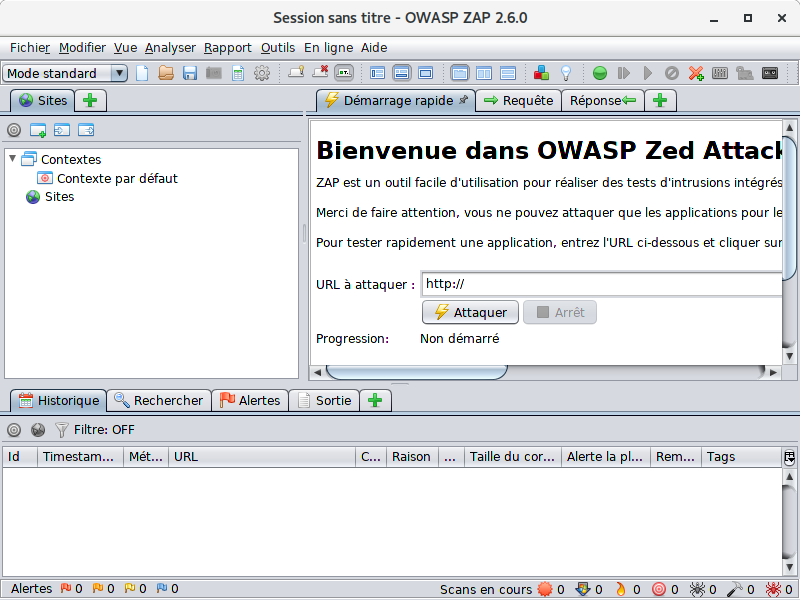
\includegraphics[width=\textwidth]{images/zap_acceuil}}
	\centering
	\caption{Fenêtre de démarrage de ZAP}
	\label{fig:zap_acceuil}
\end{figure}
ZAP\cite{zap} (voir figure~\ref{fig:zap_acceuil}) est un projet open source développé par l'OWASP\cite{owasp}. Il s'agit un proxy qui peut intercepter et analyse le trafic qui traverse la machine hôte. ZAP est un outil de sécurité très intéressant et ce pour un grand nombre de raisons :
\begin{itemize}[label=$\bullet$]
	\item activement développé\cite{zap_git} ;
	\item open source et cross-platform ;
	\item OWASP est une référence dans le monde de la sécurité ;
	\item une large communauté, et donc une grande quantité de ressources sur laquelle s'appuyer ;
	\item ZAP est contrôlable en ligne de commande (voir extrait~\ref{lst:zap_options}) et \textit{via} des APIs en plusieurs langages.
\end{itemize}

\begin{minipage}{\linewidth}
	\begin{lstlisting}[caption={Options de ZAP en ligne de commande},label={lst:zap_options},numbers=none]
$ zap.sh -cmd -help
Usage:
    zap.sh [Options]
Core options:
    -version                 Reports the ZAP version
    -cmd                     Run inline (exits when command line options complete)
    -daemon                  Starts ZAP in daemon mode, ie without a UI
    -config <kvpair>         Overrides the specified key=value pair in the configuration file
    -configfile <path>       Overrides the key=value pairs with those in the specified properties file
    -dir <dir>               Uses the specified directory instead of the default one
    -installdir <dir>        Overrides the code that detects where ZAP has been installed with the specified directory
    -h                       Shows all of the command line options available, including those added by add-ons
    -help                    The same as -h
    -newsession <path>       Creates a new session at the given location
    -session <path>          Opens the given session after starting ZAP
    -host <host>             Overrides the host used for proxying specified in the configuration file
    -port <port>             Overrides the port used for proxying specified in the configuration file
    -lowmem                  Use the database instead of memory as much as possible - this is still experimental
    -experimentaldb          Use the experimental generic database code, which is not surprisingly also still experimental
    -nostdout                Disables the default logging through standard output
Add-on options:
    -script <script>         Run the specified script from commandline or load in GUI
    -addoninstall <addon>    Install the specified add-on from the ZAP Marketplace
    -addoninstallall         Install all available add-ons from the ZAP Marketplace
    -addonuninstall <addon>  Uninstall the specified add-on
    -addonupdate             Update all changed add-ons from the ZAP Marketplace
    -addonlist               List all of the installed add-ons
    -quickurl [target url]: The URL to attack, eg http://www.example.com
    -quickout [output filename]: The file to write the XML results to
    -quickprogress: Display progress bars while scanning
    -last_scan_report <path> Generate the 'Last Scan Report' into the specified path
\end{lstlisting}
\end{minipage}

Je n'avais, avant mon stage, que brièvement eu l'occasion d'utiliser ZAP, au-travers du sous-projet de tests d'intrusion avec M. Pachy. Pouvoir m'entraîner plus longuement avec représentait donc à la fois un intérêt personnel, car cela me permettait d'en apprendre plus sur les vulnérabilités web les plus répandues, et professionnel car c'est un outil dont l'usage pourrait être pertinent pour mes futurs emplois.

ZAP est le seul outil sur lequel il y a vraiment eu un choix à faire car les tests de sécurité n'étaient pas encore implémentés à mon arrivée. Le principal concurrent de ZAP est Burp Suite\cite{burp}, une solution non-libre mais qui dispose d'une version gratuite.

Les arguments qui ont fait pencher la balance en la faveur de ZAP sont :
\begin{itemize}[label=$\bullet$]
	\item le fait que l'OWASP est une référence dans le monde de la sécurité ;
	\item le développement ouvert qui est une assurance de qualité dans le monde de la sécurité (possibilité de relever les failles/oublis/erreurs dans le code) ;
	\item le fait que moi comme mon tuteur ayons déjà eu une expérience avec ZAP et pas avec Burp.
\end{itemize}

\subsubsection{Docker}
Docker\cite{docker} est une technologie de virtualisation basée sur des conteneurs, qui vient se place en opposition aux hyperviseurs et machines virtuelles\footnote{Ou VMs pour Virtual Machines}. En plus d'une charte graphique à base de faune marine des plus plaisantes\footnote{\url{https://www.docker.com/sites/default/files/group_5622_0.png}}, la technologie Docker présente plusieurs fonctionnalités qui la rendent intéressante dans le monde de l'industrie informatique :
\begin{itemize}[label=$\bullet$]
	\item un conteneur est plus léger qu'une VM ;
	\item un conteneur s'exécute de la même façon sur n'importe quelle machine où Docker est installé ;
	\item un conteneur peut embarquer toute la configuration nécessaire au bon fonctionnement de l'application, et c'est là le point le plus important. L'étape de configuration de l'environnement n'a à être effectuée qu'une seule fois, à la création de l'image\footnote{On ne parle de conteneur qu'une fois l'image en cours d'exécution, cf. différence entre processus et programme}. De plus le système de Docker Store\cite{docker_store}, proche de celui d'un gestionnaire de paquets, permet au client d'avoir facilement la dernière version possible d'un logiciel, encore une fois en s'abstrayant des changements de configuration qui vont avec la mise-à-jour.
\end{itemize}

On assiste donc à une généralisation de l'utilisation de Docker depuis sa première version en 2013, avec de nombreux cas d'utilisation\cite{docker_use_cases}, mais aussi à une multiplication des outils en lien avec la technologie Docker comme des outils de gestion de groupes de containers\cite{kubernetes}\cite{swarm}.

GitLab-CI est étroitement lié à Docker : lors d'un push, un container est lancé dans lequel tout le processus de CI est exécuté, en isolation. De ce fait, il n'y avait pas de choix à faire quant à la technologie de virtualisation. Le comportement du processus peut être configuré au-travers d'un script en YAML, il est par exemple possible de sélectionner l'image Docker servant d'environnement d'exécution.

\subsubsection{YAML}
YAML Ain't Markup Language\cite{yaml}, de son nom complet, est un \og standard de sérialisation de données \fg. L'objectif de ce langage est de permettre de représenter des donnes à la fois clairement et simplement, principalement en les formatant comme des listes ou des maps.

La syntaxe de YAML est donc sans surprise concise et facile de prise en main\cite{yaml_refcard} ; qui plus est le code YAML est assez proche de l'anglais pour être compréhensible même par quelqu'un qui n'y est pas familier.

Dans le cas qui nous occupe, YAML est le langage permettant de contrôler le processus de CI proposé par GitLab-CI grâce à un script nommé \verb|.gitlab-ci.yml| placé à la racine du projet (l'extrait~\ref{lst:yaml_ci} est un exemple écourté de script YAML sur lequel j'ai travaillé).

\begin{minipage}{\linewidth}
	\begin{lstlisting}[caption={Script de contrôle de processus de CI en YAML},label={lst:yaml_ci}]
variables:
    MYSQL_DATABASE: database_name

services:
    - mysql:latest
    - redis:latest

deploy:
    stage: build
    image: aleonardi/symfony-mysqlclient
    stage: build
    script:
        - bash .gitlab-ci.sh
        - chmod a+x vendor/bin/phpunit
        - php vendor/bin/phpunit --colors

zap-docker:
    stage: test
    image: owasp/zap2docker-weekly:latest
    script:
        - python zap-baseline.py -t http://rick.alter-frame.fr/ -c zap.conf
    artifacts:
        - ./zap-report
    only:
        - master
        - tags
    \end{lstlisting}
\end{minipage}

\subsection{Développement Java}
Il y a moins à dire sur le développement Java car il s'agit d'un pan de travail très proche de ce que j'ai déjà rencontré par le passé, que ce soit dans des cours ou dans mon précédent stage. Chez Alter Frame, j'ai développé en Java 7 couplé à Swing pour la GUI, le tout dans un environnement Windows en utilisant les classiques Maven et git.

Encore une fois, le projet ne m'ayant pas attendu pour en premier lieu, il n'y avait pas de grande marge de manoeuvre quand à quelles technologies utiliser. L'environnement Windows est indépendant de Java à proprement parler, mais dû à l'utilisation de VBScript pour créer et modifier des classeurs Microsoft Excel.

L'incompatibilité entre le projet et Java 8 reste, elle, un mystère\footnote{\url{https://i.pinimg.com/564x/66/ba/a0/66baa08b16a192d752959fa4c29bc96a.jpg}}.
%\footnote{\url{https://xkcd.com/722/}}.

\subsection{Audit technique}
\subsubsection{ZAP : Zed Attack Proxy}
J'ai à nouveau eu l'occasion d'utiliser ZAP pendant le déroulement de l'audit. Cette fois-ci il ne s'agissait pas d'en automatiser l'usage et donc de le contrôler au-travers d'une API, mais bien d'un cas d'usage plus classique où j'ai configuré ZAP comme proxy Internet, et observé le trafic lors de l'utilisation de l'application auditée grâce à son interface graphique.

Néanmoins, les avantages de ZAP qui ont fait que mon tuteur et moi l'avons retenu pour l'intégration continue s'appliquent toujours ici (excepté pour le contrôle par API/ligne de commande) et le raison du choix de ZAP est donc la même.

\subsubsection{SonarQube}
SonarQube est un outil d'analyse de code bien connu. Bien que sa vocation première soit d'améliorer la qualité et la maintenabilité du code analysé, Sonar incorpore aussi des règles de sécurité dans ses patrons de détection. C'est dans cette optique que je l'ai utilisé (la figure~\ref{fig:sonar_sec} liste une partie des vulnérabilités que sait détecter Sonar).

\begin{figure}{l}
	\makebox[\textwidth][c]{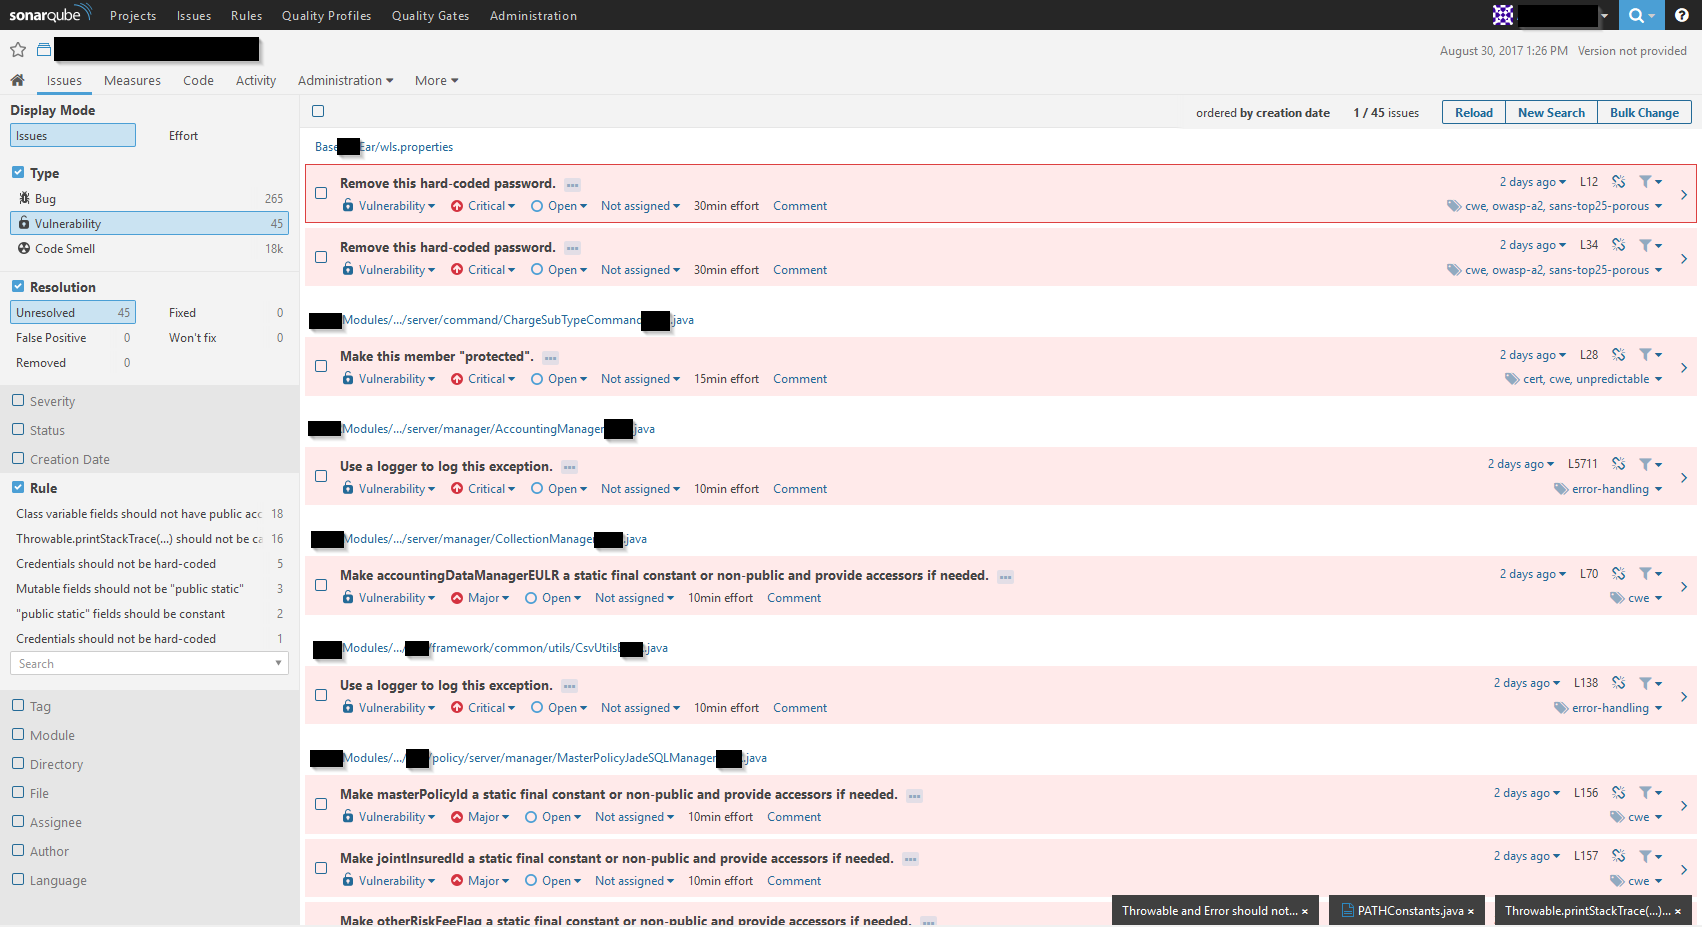
\includegraphics[width=\paperwidth]{images/sonar_sec_audit}}
	\caption{Extrait des résultats de sécurité du scanner Sonar}
	\label{fig:sonar_sec}
\end{figure}

C'est durant l'audit que j'ai majoritairement utilisé Sonar, mais les scripts de CI qui étaient en plus avant mon arrivée chez Alter Frame incorporaient déjà des analyses Sonar effectuées sur le code. C'est d'ailleurs de ce fait (mon tuteur ayant déjà de l'expérience avec ce logiciel) ainsi que du faible nombre de concurrents gratuits\cite{squale} que nous avons choisi d'utiliser Sonar dans ce cas de figure.

\subsubsection{JMeter \& SoapUI}
Ces deux outils, de même que ZAP, avaient déjà été utilisés lors des itérations précédentes de l'audit, et les conserver permettait de comparer facilement les résultats que nous obtiendrions avec les résultats antérieurs. Aussi, en l'absence de raison de ne \emph{pas} les conserver, nous les avons conservés.

SoapUI\cite{soapui} est un outil de test pour applications REST ou SOAP. L'application auditée utilisait le protocole SOAP, et SoapUI nous a servi à modifier et rejouer des requêtes isolées, sans tester les performances de l'application mais pour en saisir le fonctionnement et préparer le véritable test, en plus de vérifier que nous avions bien les droits pour réaliser toutes les opérations prévues.

JMeter est un outil de test de performances pour applications web en général. Le panel de fonctionnalités qu'il offre est extrêmement large (et en conséquence, sa prise en main est loin d'être triviale) et nous n'en avons utilisé qu'une partie : configurer JMeter comme proxy pour enregistrer un cas d'utilisation typique qui servira de scénario de test (on peut voir les différentes étapes d'un tel scénario dans l'interface de JMeter dans la figure~\ref{fig:jmeter}), puis rejouer celui-ci en boucle et plusieurs fois en parallèle pour tester les limites de l'application.
\begin{figure}
  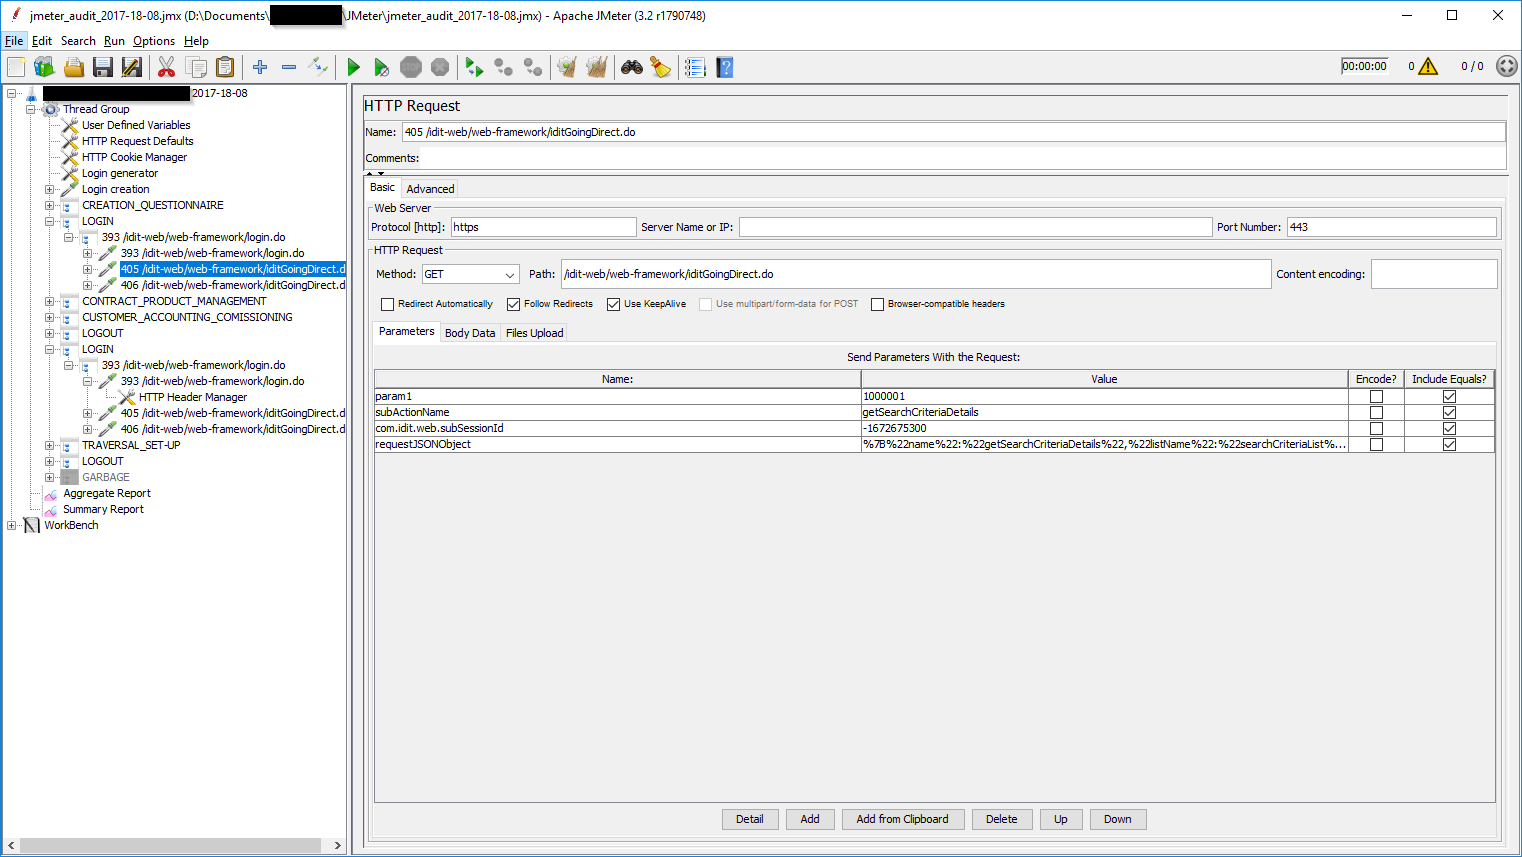
\includegraphics[width=\linewidth]{images/jmeter}
  \caption{JMeter, une fois configuré}
  \label{fig:jmeter}
\end{figure}

%TODO: ajouter un screen de JMeter
%%% Local Variables:
%%% mode: latex
%%% TeX-master: "../M2FSI-rapport-LEONARDI-alexandre"
%%% End:

\pagebreak
\section{Synthèse du travail d'intégration continue}
\label{sec:synthese_ci}
L'amélioration du CI d'Alter-Frame et l'ajout de la composante sécurité a été la tâche principale de mon stage.

Un point sur le fonctionnement et la nomenclature de GitLab-CI\cite{gitlab_ci_workflow} : le script de contrôle du processus de CI est le \texttt{.gitlab-ci.yml}, ou le \texttt{.yml} pour faire court. Le comportement par défaut pour ce script est de définir une image Docker, avec la balise \texttt{image} (on aurait par exemple \texttt{image: openjdk:latest} pour aller chercher l'image openjdk sur le hub docker, et récupérer la version taguée "latest").

Cette image va être instanciée en un container au début de l'exécution du script, et ce dernier se déroulera dans l'environnement du container. Utiliser l'image openjdk par exemple donne accès à une JDK et permet donc d'appeler des fonctions telles que javac ou d'installer des utilitaires qui en dépendent tels que SonarQube.

On appelle "runner" l'hôte sur lequel s'exécute l'image docker, et "job" chacune des fonctions en lesquelles le script peut être séparé. Eux-mêmes peuvent être regroupés en stages : les stages s'exécutent dans l'ordre dans lequel ils sont déclarés et si un stage échoue, le runner s'arrête. En revanche, l'ordre des jobs au sein d'un stage est à la discrétion du runner et ne peut pas être connu.

La figure~\ref{fig:ci_flow} résume le fonctionnement de GitLab-CI.

\begin{figure}
	\centering
	\caption{Résumé du processus de CI (\emph{build}, \emph{test} et \emph{deploy} sont les stages par défaut)}
	\label{fig:ci_process}
	\frame{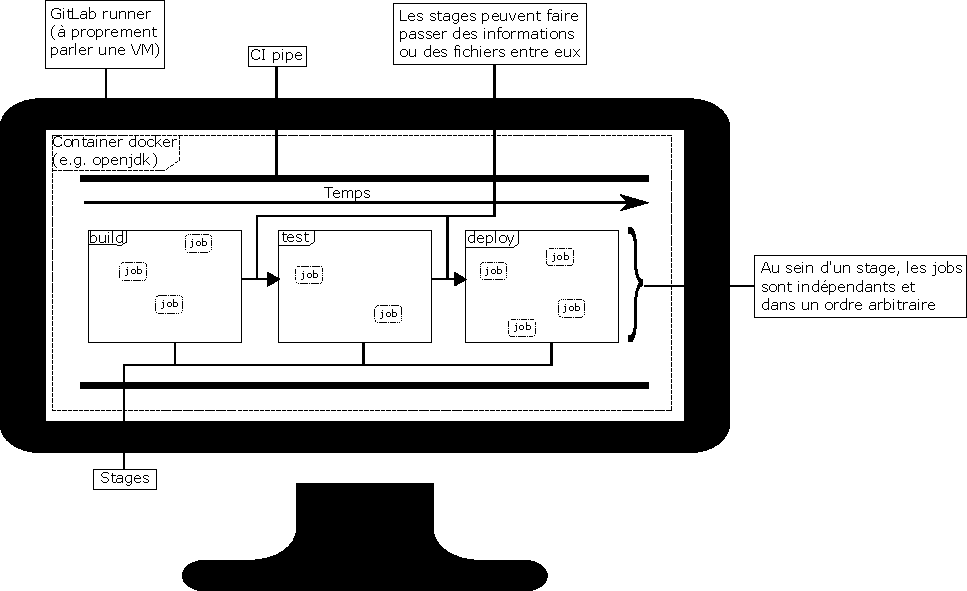
\includegraphics[width=\textwidth]{images/process_ci.pdf}}
\end{figure}

\subsection{Déployer automatiquement les applications web}
Mon intervention sur cette partie a été en commun avec un autre ingénieur d'Alter Frame. Nous devions faire en sorte de compiler les applications web en PHP, et générer à partir de là une image Docker contenant l'application et toute la configuration requise, puis  déployer cette image sur un serveur appartenant à Alter Frame.

Voilà pour la théorie. La pratique a été une succession d'approches différentes qui n'ont pas toujours été fructueuses, et beaucoup d'essai et échec permettant d'avancer petit à petit ; il faut savoir que la documentation de GitLab-CI sur le sujet\cite{gitlab_docker_build} n'est pas parfaitement complète et fait la supposition que l'utilisateur possède une bonne connaissance de Docker.

La première approche fut d'exécuter le runner en mode shell plutôt que Docker. C'est la méthode la plus facile mais aussi celle qui s'éloigne le plus du comportement par défaut et qui fait perdre la grande flexibilité qu'offre le fonctionnement par image Docker : les différents outils doivent être définitivement installés sur le serveur qui héberge les runners.

En plus de ce défaut, cette méthode est discutable d'un point de vue sécurité car elle exige que l'utilisateur qui exécute le script ait des privilèges administrateur, donc indirectement toute personne qui intervient sur les scripts .yml\footnote{Un article sur la sécurité du groupe Docker : \url{https://www.andreas-jung.com/contents/on-docker-security-docker-group-considered-harmful}}.

Au final et malgré ses points négatifs, cette méthode nous a permis d'arriver à nos fins, mais nous ne l'avons pas retenue, pour partie pour les raisons exposées plus haut et pour partie pour des raisons propres à la compilation de l'application en PHP qui bloquaient l'ingénieur avec lequel j'ai travaillé.

Deuxième approche, plus en accord avec la philosophie de GitLab-CI : utiliser docker-in-docker (dind). L'idée est simple et la mise en oeuvre plus complexe (pour changer). Il s'agit de fournir au runner une image disposant des utilitaires nécessaires pour construire une image docker, et finalement de réaliser le même processus qu'en mode shell, mais dans le contexte isolé du container docker parent.

Les inconvénients de la méthode shell disparaissent : plus besoin d'installer en dur sur le serveur des utilitaires qui sont spécifiques à un projet (le serveur héberge plusieurs runners qui se répartissent tous les projets d'Alter Frame selon les besoins) ; plus besoin non plus d'avoir des privilièges administrateur sur le serveur.

Bien entendu cette méthode aussi avait un coût. Tout d'abord, GitLab-CI met en place des protections pour éviter que tout développeur puisse, par défaut, avoir accès à ces fonctionnalités et il faut donc une étape de configuration supplémentaire au niveau des runners pour utiliser dind.

Ensuite, déployer et configurer une application est un procédé lourd qui peut impliquer l'installation de dépendances. En réalisant cela dans un container, deux cas de figure se présentent :
\begin{itemize}[label=$\bullet$]
	\item soit on utilise une image générique proposant l'outil de base (e.g. openjdk:latest pour un projet Java) et on installe dans le .yml les différentes dépendance. Ce n'est pas compliqué de mise en oeuvre, mais chaque exécution du script sera longue, et la lenteur est vite limitante dans le domaine de l'intégration continue (le développeur n'a pas toujours le temps d'attendre qu'un procédé long se termine) ;
	\item soit on crée une image personnalisée qui embarque déjà les dépendances requises, cela accélère le processus de CI mais rajoute du travail en amont avec la création et la configuration de l'image, ainsi que son stockage sur un registre Docker. De plus, le processus perd en transparence car la configuration de l'environnement devient cachée au développeur qui ne voit que le nom de l'image utilisée. Bien sûr, cela peut aussi être vu comme un avantage car le .yml s'en trouve d'autant allégé, et ne contient au final plus que l'essentiel du point de vue intégration et déploiement.
\end{itemize}
\begin{minipage}{\linewidth}
	\begin{lstlisting}[caption={Dockerfile utilisé pour le job de déploiement de l'application},label={lst:dockerfile}]
		FROM nouchka/symfony:7.0
		LABEL maintainer="aleonardi@alter-frame.com"
		
		ARG mysql_apt_version
		
		ENV DEBIAN_FRONTEND=noninteractive
		ENV DEBCONF_NONINTERACTIVE_SEEN=true
		
		RUN apt-get update -yqq
		RUN apt-get install --assume-yes wget lsb-release gnupg
		RUN wget https://dev.mysql.com/get/mysql-apt-config_${mysql_apt_version}_all.deb
		RUN dpkg -i mysql-apt-config_${mysql_apt_version}_all.deb
		RUN apt-get update -yqq
		RUN apt-get install --assume-yes mysql-client		
\end{lstlisting}
\end{minipage}

C'est la deuxième approche que j'ai conservée (voir le code de l'image en question dans le listing~\ref{lst:dockerfile}), mais non sans avoir testé la première au préalable. Avoir la configuration directement dans le .yml était source de complexité (appeler un .sh à l'intérieur du .yml pour externaliser de gros blocs de code) et de bugs (de petits changements pouvaient entraîner des résultats inattendus, surtout compte tenu du fait que nous étions plusieurs à intervenir sur le .yml).

Au final, cette méthode a tenu ses promesses : nous nous retrouvions avec une configuration sauvegardée à part, facile et rapide à importer, et qui comportait toutes les dépendances requises pour le projet. De plus un runner avait été spécialement configuré pour permettre l'utilisation de dind, restreinte par défaut, et générer l'image qui encapsulait l'appli web développée par Alter Frame devenait possible.

\subsection{Intégrer ZAP et les analyses de sécurité}
ZAP a pour lui d'intégrer par défaut les cas d'usage qui m'importaient, à savoir de pouvoir être utilisé en mode ligne de commade et/ou contrôlé par une API sans interaction avec l'utilisateur au moment de l'exécution.

De ces deux solutions, c'est celle de l'API qui est la plus complète : ZAP en ligne de commande propose quelques options (cf. listing~\ref{lst:zap_options}) mais qui sont vite limitées : se connecter à un site web, lancer certaines des commandes de base de l'application comme le crawler ou le scan actif, et générer un fichier de résultats. Le scan actif de ZAP est tout de même assez intéressant pour que cette méthode soit pertinente, mais les options proposées par les APIs sont bien plus foisonnantes.

Néanmoins, la solution de l'API rajoute une contrainte : en plus de ZAP, il faut que l'environnement de CI dispose du langage de l'API. Les deux APIs principales maintenues par la communauté de développeurs ``officiels'' de ZAP sont celles en Java et en Python. J'ai retenu l'utilisation de Python d'une part car ce langage est concis et se prête très bien à l'écriture de courts scripts, d'autre part pour avoir l'occasion de m'en servir et développer des compétences qui me seraient utiles plus tard dans mon parcours professionnel (ce qui sera le cas dès octobre, cf section~\ref{sec:avenir}).

Plutôt que de rajouter encore un élément à l'image Docker créée spécialement au point précédent, j'ai préféré utiliser une fonctionnalité très intéressante de GitLab-CI, celle de pouvoir spécifier une image différente pour chaque job. Elle rajoute en verbosité au script car l'image doit donc être spécifiée pour chaque job sans exception (impossible d'en utiliser une par défaut et de ne la remplacer que pour le job de l'analyse ZAP), mais elle évite de surcharger l'image Docker utilisée pour le déploiement. Qui plus est, cette image de déploiement est spécifique à chaque projet et doit donc être réécrire, alors que le script commandant l'exécution de ZAP peut être générique (exception faite de l'URL cible). Inclure l'image à utiliser à ce script renforce cette autonomie, le bloc de code peut littéralement être copié collé d'un projet à l'autre et fonctionner (encore une fois sous réserve de changer l'URL à attaquer).
% TODO : inclure le snippet de ZAP

Nous nous retrouvons avec une configuration versatile : elle peut être exportée facilement et profite de toute l'expressivité de l'API Python pour ZAP. L'OWASP propose des images Docker de ZAP\footnote{\href{https://github.com/zaproxy/zaproxy/wiki/Docker}{La page du wiki correspondante} et \href{https://github.com/zaproxy/zaproxy/tree/develop/build/docker}{le dépôt avec les Dockerfiles}} mais elles ne correspondent pas à mon besoin, elles exposent un script nommé zap-scanner qui permet, comme son nom l'indique, de lancer un scanner ZAP en ligne de commande. Pour une utilisation dans le cadre de GitLab-CI, on cherche plutôt des images qui exposent /bin/sh, car cela signifie qu'une fois le container lancé on à accès à /bin/sh et on peut donc utiliser la ligne de commande.

Bien sûr il existe des images non officielles de ZAP\footnote{E.g. une image pour utiliser ZAP comme un \textit{goal} Maven : \url{https://github.com/pdsoftplan/zap-maven-plugin}} mais qui, à chaque fois, ont été créées avec un usage précis en tête plutôt que dans un but de généricité ou n'étaient plus maintenues et ne correspondaient donc, encore une fois, pas à mon besoin. La conséquence a été que j'ai utilisé une image générique qui ne contient que Python et une installation Linux basique\footnote{à savoir \href{https://github.com/docker-library/python/blob/d3c5f47b788adb96e69477dadfb0baca1d97f764/3.3/alpine3.4/Dockerfile}{python:3.3.6-alpine3.4}, qui a l'avantage d'être plus légère que \href{https://github.com/docker-library/python/blob/d3c5f47b788adb96e69477dadfb0baca1d97f764/3.6/jessie/Dockerfile}{python:latest} qui utilise Debian.}, et j'ai installé \textit{via} le .yml ZAP. Le script Python pour contrôler l'attaque était inclus dans le dépôt git, et il ne restait plus qu'à l'appeler en spécifiant, en paramètre, l'URL à attaquer.

\begin{figure}[h]
	\centering
	\caption{Récapitulatif du \textit{build} et icône de téléchargement du rapport ZAP}
	\label{fig:gitlab_build_recap}
	\frame{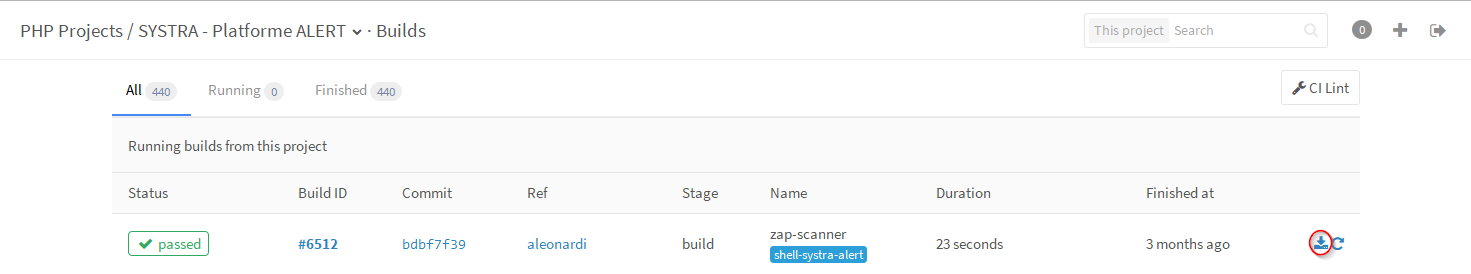
\includegraphics[width=\textwidth]{images/gitlab_build_recap}}
\end{figure}

La dernière étape était de générer, et rendre disponible, un rapport pour que les développeurs puissent prendre des mesures. L'idéal aurait été d'envoyer automatiquement un mail à l'auteur du commit et qui contiendrait le rapport en XML, néanmoins le temps ne m'a pas permis de me pencher sur la faisabilité de cette fonctionnalité. Ce que j'ai  fait en revanche est de créer un artefact, c'est-à-dire de marquer un fichier généré pendant le job comme persistant pour que GitLab le sauvegarder sur le serveur qui héberge les runners et le rende téléchargeable dans son interface web. Un example de la syntaxe utilisée est visible dans le listing~\ref{lst:zap-report}.

\begin{minipage}{\linewidth}
	\begin{lstlisting}[caption={Extrait de code qui lance un scanner ZAP en ligne de commande et rend le rapport disponible sur GitLab},label={lst:zap-report}]
		zap-scanner:
		stage: test
		script:
			- # ...
				# The output file has to be specified here, otherwise it will be printed on standard output
			- docker exec zap-sh zap-cli -p 8090 active-scan 'http://itsecgames.com/' > zap-report.xml 
			- # ...
		artifacts:
			paths:
				# The path to the report has to be specified here to be downloadable 
			- ./zap-report.xml
\end{lstlisting}
\end{minipage}

Dans l'interface web de GitLab, le détail des résultats des builds sont visibles dans une page à part où le rapport peut-être téléchargé (l'icône entourée en rouge dans la figure~\ref{fig:gitlab_build_recap}).

\subsection{Amélioration de l'existant}
Les deux points précédents étaient des ajouts et, de ce fait, la part la plus visible de mon travail sur le processus de CI, mais une partie en était déjà établie à mon arrivée et j'ai aussi travaillé sur cette partie, pour l'améliorer : principalement du point de vue de la lisibilité et de la maintenabilité.

On peut résumer mon intervention en trois points importants :

\begin{itemize}[label=$\bullet$]
	\item regrouper le code dupliqué et utiliser des ancres\footnote{\url{https://docs.gitlab.com/ee/ci/yaml/\#anchors}} et des templates (cf. listing~\ref{lst:anchor}) ;
	\item utiliser des images Docker pré-configurées plutôt que télécharger et installer un logiciel, autant que possible ;
	\item stocker les valeurs variables (numéro de version, identifiants de connexion, etc) dans des variables (précisément). À noter que GitLab-CI offre une mécanique de variables secrètes\footnote{\url{https://docs.gitlab.com/ee/ci/variables/\#secret-variables}}.
\end{itemize}

\begin{minipage}{\linewidth}
	\begin{lstlisting}[caption={Template d'installation et utilisation de Maven, et son appel dans un job},label={lst:anchor}]
		## Template for building code
		.build_template: &maven_clean_install
			script:
				## Install maven
				- wget -q http://wwwftp.ciril.fr/pub/apache/maven/maven-${MAVEN_MAJOR_VERSION}/${MAVEN_FULL_VERSION}/binaries/apache-maven-${MAVEN_FULL_VERSION}-bin.zip
				- unzip -qq apache-maven-${MAVEN_FULL_VERSION}-bin.zip
				- rm apache-maven-${MAVEN_FULL_VERSION}-bin.zip
			
				## Install and populate database
				- export
				- apt-get update && apt-get --assume-yes install mysql-client
				- mysql --user=$MYSQL_ROOT_USERNAME --password="$MYSQL_ROOT_PASSWORD" --host=mysql "$MYSQL_DATABASE" < ./server/sql/db-structure.sql
				
				## Build application
				- ./apache-maven-${MAVEN_FULL_VERSION}/bin/mvn -f ./root/pom.xml clean install

				mvn:
				stage: build
				## Importing services
				services: *mysql
				## Merging anchored code with current job
				<<: *maven_clean_install
				only:
					- develop
\end{lstlisting}
\end{minipage}
\pagebreak
\section{Synthèse du développement Java}
\label{sec:synthese_java}

\subsection{Méthodologie}
\subsection{Travail effectué}
\pagebreak
\section{Synthèse de l'audit}
\label{sec:synthese_audit}

\subsection{Méthodologie}
\subsection{Travail effectué}
\pagebreak
\section*{Conclusion}

Penser à mettre les crédits pour le template
\pagebreak
\listoffigures
\pagebreak
\lstlistoflistings
\pagebreak
\printbibliography

\end{document}